%%
% BIThesis 本科毕业设计论文模板 —— 使用 XeLaTeX 编译 The BIThesis Template for Undergraduate Thesis
% This file has no copyright assigned and is placed in the Public Domain.
%%

\chapter{动态场景的无人机集群动力学建模}

\section{引言}
在非全维位置量测条件下实现无人机集群的稳定编队控制，其核心挑战在于如何构建一个既能准确反映系统物理特性，又便于进行后续可观测性分析与控制器设计的数学模型。实际应用中的四旋翼无人机是典型的欠驱动、强耦合非线性系统，其完整的六自由度动力学模型极为复杂。此外，受限于机载计算平台的算力资源，高维非线性模型直接应用于大规模集群的分布式协同控制时，难以满足系统对实时性与计算效率的严苛要求\cite{2014Programmable}。若直接在此基础上进行分布式协同控制设计，不仅会因高维非线性而难以分析系统的可观测性，更会使控制器的设计与实现变得异常繁琐，甚至不可行。

为应对上述挑战，本章旨在构建一套面向协同控制任务的无人机集群动力学建模框架，在保留系统核心运动特性的前提下实现模型降阶。具体而言，本章工作将围绕以下两个关键方面展开。首先，基于无人机普遍采用的内外环分层控制架构，对系统进行解耦处理。通过将底层的姿态控制环视为快速响应的执行单元，我们得以将顶层的编队协同问题从复杂的姿态动力学中剥离出来，并在平衡点附近对简化的运动学模型进行线性化，从而获得一个易于处理的二阶积分器质点模型。其次，为了刻画集群中信息交互的结构特性，我们将引入图论作为数学工具，对无人机节点间的通信拓扑结构进行形式化描述。这为后续分析编队刚性、系统可观测性以及设计分布式观测与控制律奠定了坚实的理论基础。

值得注意的是，针对量测受限的场景，已有研究取得了重要进展。例如，黄山等人\parencite{HKXB202413019}针对GPS拒止环境，提出了一种仅利用距离量测即可实现多无人机对未知目标协同环绕的控制方法，有效解决了目标位置信息完全未知的难题。这充分说明了在特定任务下，通过精巧的算法设计，可以克服传感器信息的不足。然而，对于更一般的编队飞行任务，尤其是在部分无人机仅有非全维绝对位置、部分仅有相对距离的异构量测条件下，如何建立统一的建模与分析框架仍是亟待解决的问题。因此，本章的核心目的正是构建一个“简化动力学-通信拓扑”一体化的建模框架。该框架在保留编队协同控制本质特征的同时，极大地降低了问题的复杂度，为第三章及以后关于非全维量测下系统可观测性分析、分布式状态观测器设计和鲁棒协同控制器构建等核心研究内容提供了必要且坚实的模型支撑。

\section{四旋翼无人机动力学模型}
本节将对四旋翼无人机动力学建模方法展开讨论。四旋翼无人机本质上是一个具有六自由度的强非线性、欠驱动系统，其姿态动力学与平移动力学之间存在紧密耦合。机体的姿态变化直接决定了推力在惯性系中的投影方向，从而影响位置运动；而位置控制指令又需通过调整姿态来实现。这种复杂的耦合特性使得基于完整非线性模型的协同控制器设计不仅计算负担重，而且难以保证实时性与鲁棒性，尤其在机载资源受限的集群应用场景中尤为突出。为兼顾模型精度与控制可实现性，本文引入内外环解耦的建模思想。姿态环作为内环负责快速跟踪期望姿态角，位置姿态环作为外环则根据任务需求生成相应的姿态参考指令。通过将内环视为一个高带宽、快响应的伺服单元，可将顶层编队协同问题从底层复杂的刚体动力学中有效剥离。在此基础上，对系统在悬停或准静态平衡点附近进行小角度线性化，即可获得一个结构简洁、物理意义清晰的简化线性模型。这一简化模型不仅显著降低了控制器设计的复杂度，也为后续的系统可观测性分析、分布式状态估计以及编队稳定性证明提供了便利的数学基础，是连接高保真物理系统与高层协同算法之间的关键桥梁。

\subsection{四旋翼无人机的刚体动力学}
四旋翼飞行器作为最常见的多旋翼飞行平台，本质上是一种结构简单的装置。如图\ref{常见四旋翼飞行器}所示，它由四个独立旋翼固定在刚性十字形机身框架上构成。四旋翼的操控原理基于各旋翼产生的推力进行差动控制，俯仰、横滚和升降的控制机制则相对直观。由于系统存在欠驱动特性，$x-y$平面内平移速度对应的剩余自由度必须通过系统动力学进行控制。

\begin{figure}[H]
	\centering
	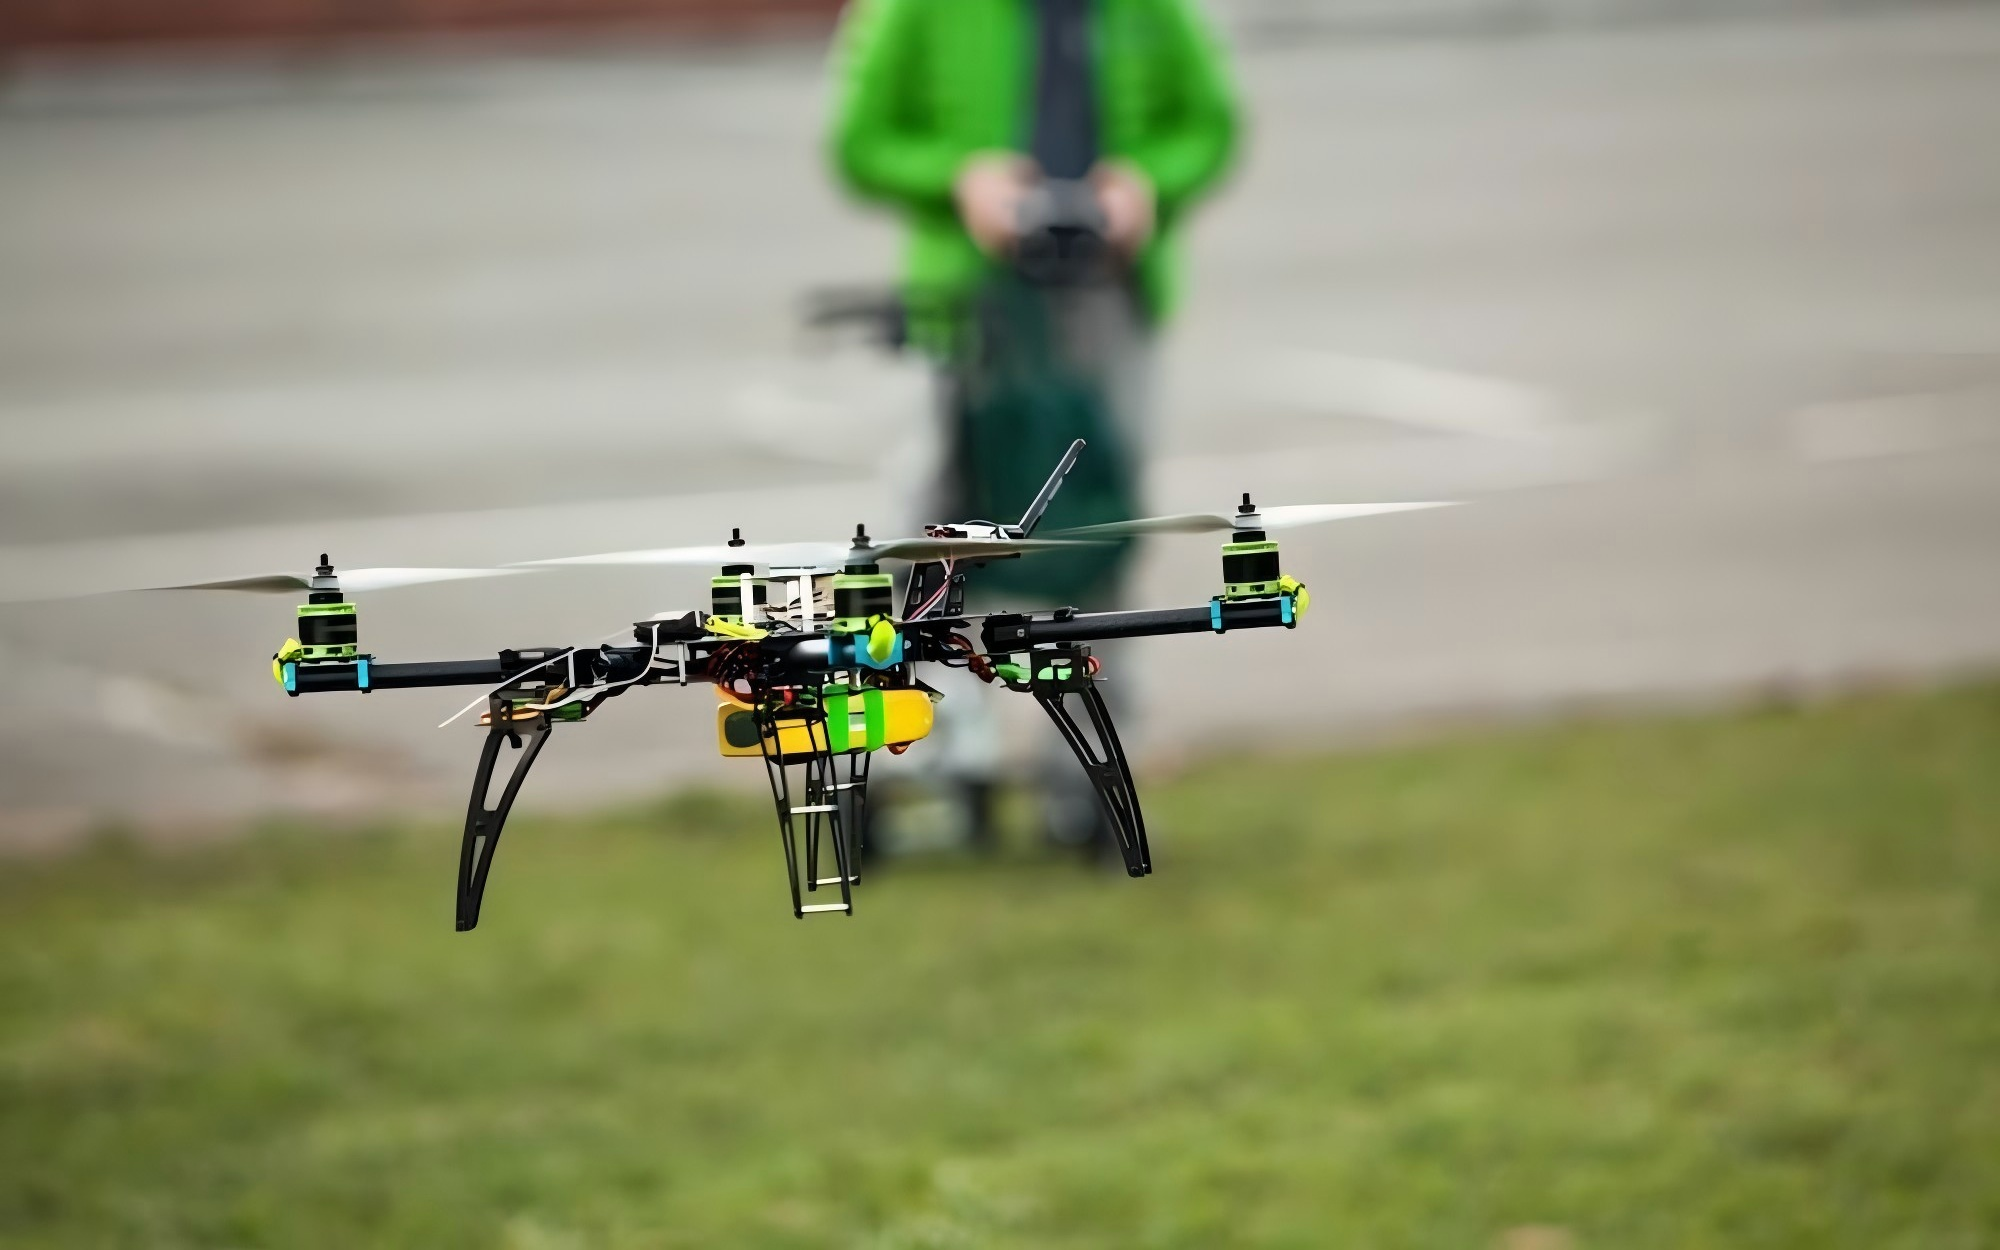
\includegraphics[width=0.5\linewidth]{images/2-1}
	\caption{常见四旋翼飞行器}
	%\vspace{-20pt}
	\label{常见四旋翼飞行器}
\end{figure}


为建立精确且通用的动力学模型，本小节参考经典文献\parencite{6289431}的方法，对四旋翼无人机进行刚体动力学建模。如图所示，我们定义一个右手惯性坐标系   $O - X_eY_eZ_e$ ，这里令地面坐标系为惯性坐标系，其单位基向量为  $ \{\mathbf{e}_1, \mathbf{e}_2, \mathbf{e}_3\} $ ；以及一个固连于无人机质心的机体坐标系  $ O - X_bY_bZ_b $ ，其单位基向量为  $ \{\mathbf{b}_1, \mathbf{b}_2, \mathbf{b}_3\} $ 。无人机的姿态由从  $ O - X_eY_eZ_e $  到  $ O - X_bY_bZ_b $  的旋转矩阵  $ {}_b^\omega R = R = [{\mathbf{b}}_1,{\mathbf{b}}_2,{\mathbf{b}}_3]\in SO(3) $  描述。该矩阵属于特殊正交群，其中 $ \mathbf{b}_1 = R \mathbf{e}_1,  \mathbf{b}_2 = R \mathbf{e}_2, \mathbf{b}_3 = R \mathbf{e}_3 $。基于$ z-y-x $欧拉角顺序（即偏航角  $ \psi $ 、俯仰角  $ \theta $ 、滚转角  $ \phi $ ）来参数化旋转矩阵 $ \boldsymbol{R} $ ，其具体形式可写为：
\begin{equation}
	{R} = {}_b^\omega R(\phi,\theta,\psi) = 
	\begin{bmatrix}
		\mathbf{c}_\psi \mathbf{c}_\theta & 
		\mathbf{s}_\phi \mathbf{s}_\theta \mathbf{c}_\psi - \mathbf{c}_\phi \mathbf{s}_\psi & 
		\mathbf{c}_\phi \mathbf{s}_\theta \mathbf{c}_\psi + \mathbf{s}_\phi \mathbf{s}_\psi \\
		\mathbf{c}_\theta \mathbf{s}_\psi & 
		\mathbf{s}_\phi \mathbf{s}_\theta \mathbf{s}_\psi + \mathbf{c}_\phi \mathbf{c}_\psi & 
		\mathbf{c}_\phi \mathbf{s}_\theta \mathbf{s}_\psi - \mathbf{s}_\phi \mathbf{c}_\psi \\
		-\mathbf{s}_\theta & 
		\mathbf{s}_\phi \mathbf{c}_\theta  & 
		\mathbf{c}_\phi \mathbf{c}_\theta
	\end{bmatrix}.
	\label{旋转矩阵}
\end{equation}
其中  $ \mathbf{c} $  和  $ \mathbf{s} $  分别为余弦和正弦的简写，例如  $ \mathbf{c}_\psi = \cos\psi $ ,  $ \mathbf{s}_\theta = \sin\theta $  等。

设  $ \mathbf{p} = [x, y, z]^\top \in \mathbb{R}^3 $  为无人机质心在惯性系  $O - X_eY_eZ_e$  中的位置向量， $ \mathbf{v} \in \mathbb{R}^3 $  为其对应的线速度。在机体坐标系 $ O - X_bY_bZ_b $ 中定义向量  $ \boldsymbol{\Omega} \in \mathbb{R}^3 $  表示机体坐标系  $ O - X_bY_bZ_b $  相对于惯性系  $ O - X_eY_eZ_e $  的角速度。无人机的质量为  $ m $ ，其在机体坐标系下的常值转动惯量矩阵为  $ {J} \in \mathbb{R}^{3 \times 3} $ 。

基于牛顿-欧拉方程，四旋翼无人机的刚体动力学方程可表述为：
\begin{align}
	\dot{\mathbf{p}} &= \mathbf{v}, 
	\label{位置导数等于速度} \\
	m \dot{\mathbf{v}} &= m g \mathbf{e}_3 + {R} \mathbf{f}, 
	\label{平动动力学} \\
	\dot{R} &= {R} \boldsymbol{\Omega}_\times, 
	\label{姿态} \\
	{J} \dot{\boldsymbol{\Omega}} &= - \boldsymbol{\Omega} \times {J} \boldsymbol{\Omega} + \boldsymbol{\tau}.
	\label{旋转动力学}
\end{align}
其中， $ g $  为重力加速度，符号  $ (\cdot)_\times $  表示将向量映射为对应的反对称矩阵，即对于任意向量  $ \boldsymbol{x} = [x_1, x_2, x_3]^\top $ ，有
\begin{equation}
\boldsymbol{x}_\times =
\begin{bmatrix}
	0 & -x_3 & x_2 \\
	x_3 & 0 & -x_1 \\
	-x_2 & x_1 & 0
\end{bmatrix}.
\end{equation}

向量$ \mathbf{f} \in \mathbb{R}^3 $  和  $ \boldsymbol{\tau} = [\tau_1; \tau_2; \tau_3] \in \mathbb{R}^3 $  分别代表由旋翼气动效应产生的、在机体坐标系  $ O - X_bY_bZ_b $  下表示的合力与合力矩。假设无人机主要受重力与旋翼推力作用，忽略空气阻力及风场干扰，则机体坐标系下的合外力可近似表示为：
\begin{equation}
	\mathbf{f} \approx \mathit{T_f} \mathbf{e}_3. \label{合外力}
\end{equation}
式中 $ \mathit{T_f} $ 表示四个旋翼基于空气动力学产生的悬停总推力。


\subsection{四旋翼无人机的分层控制结构}
轨迹跟踪控制的核心目标是驱动无人机系统状态 $(\mathbf{p}, R)$渐近收敛至期望参考轨迹$ (\mathbf{p}^{*}(t), R^{*}(t)) \in \mathrm{SE}(3) $然而，该控制问题的求解面临欠驱动约束、模型不确定性及参数摄动等多重挑战。首先，系统存在欠驱动问题，虽然 $ \mathrm{SE}(3) $ 是六维系统，但仅有四个输入量$  u_T = \mathit{T_f} , \mathbf{u}_\tau = [\tau_1, \tau_2, \tau_3]$。其次，前述气动模型仅为近似描述。最后，输入参数本身也经过理想化处理。实际应用中，电机控制器必须克服阻力矩才能产生所需速度，并实现输入推力和力矩。尽管一阶线性模型是有效近似，但电机动力学特性及其与螺旋桨阻力的相互作用仍难以精确建模。在工程实践中，四旋翼飞行器通常采用分层控制架构。该架构通常包含三个层级：底层为电机转速控制回路，中间层为姿态镇定回路，顶层为位置/轨迹跟踪回路。这些层级形成嵌套反馈回路，如图\ref{四旋翼无人机分层控制结构}所示。

\begin{figure}[H]
	\centering
	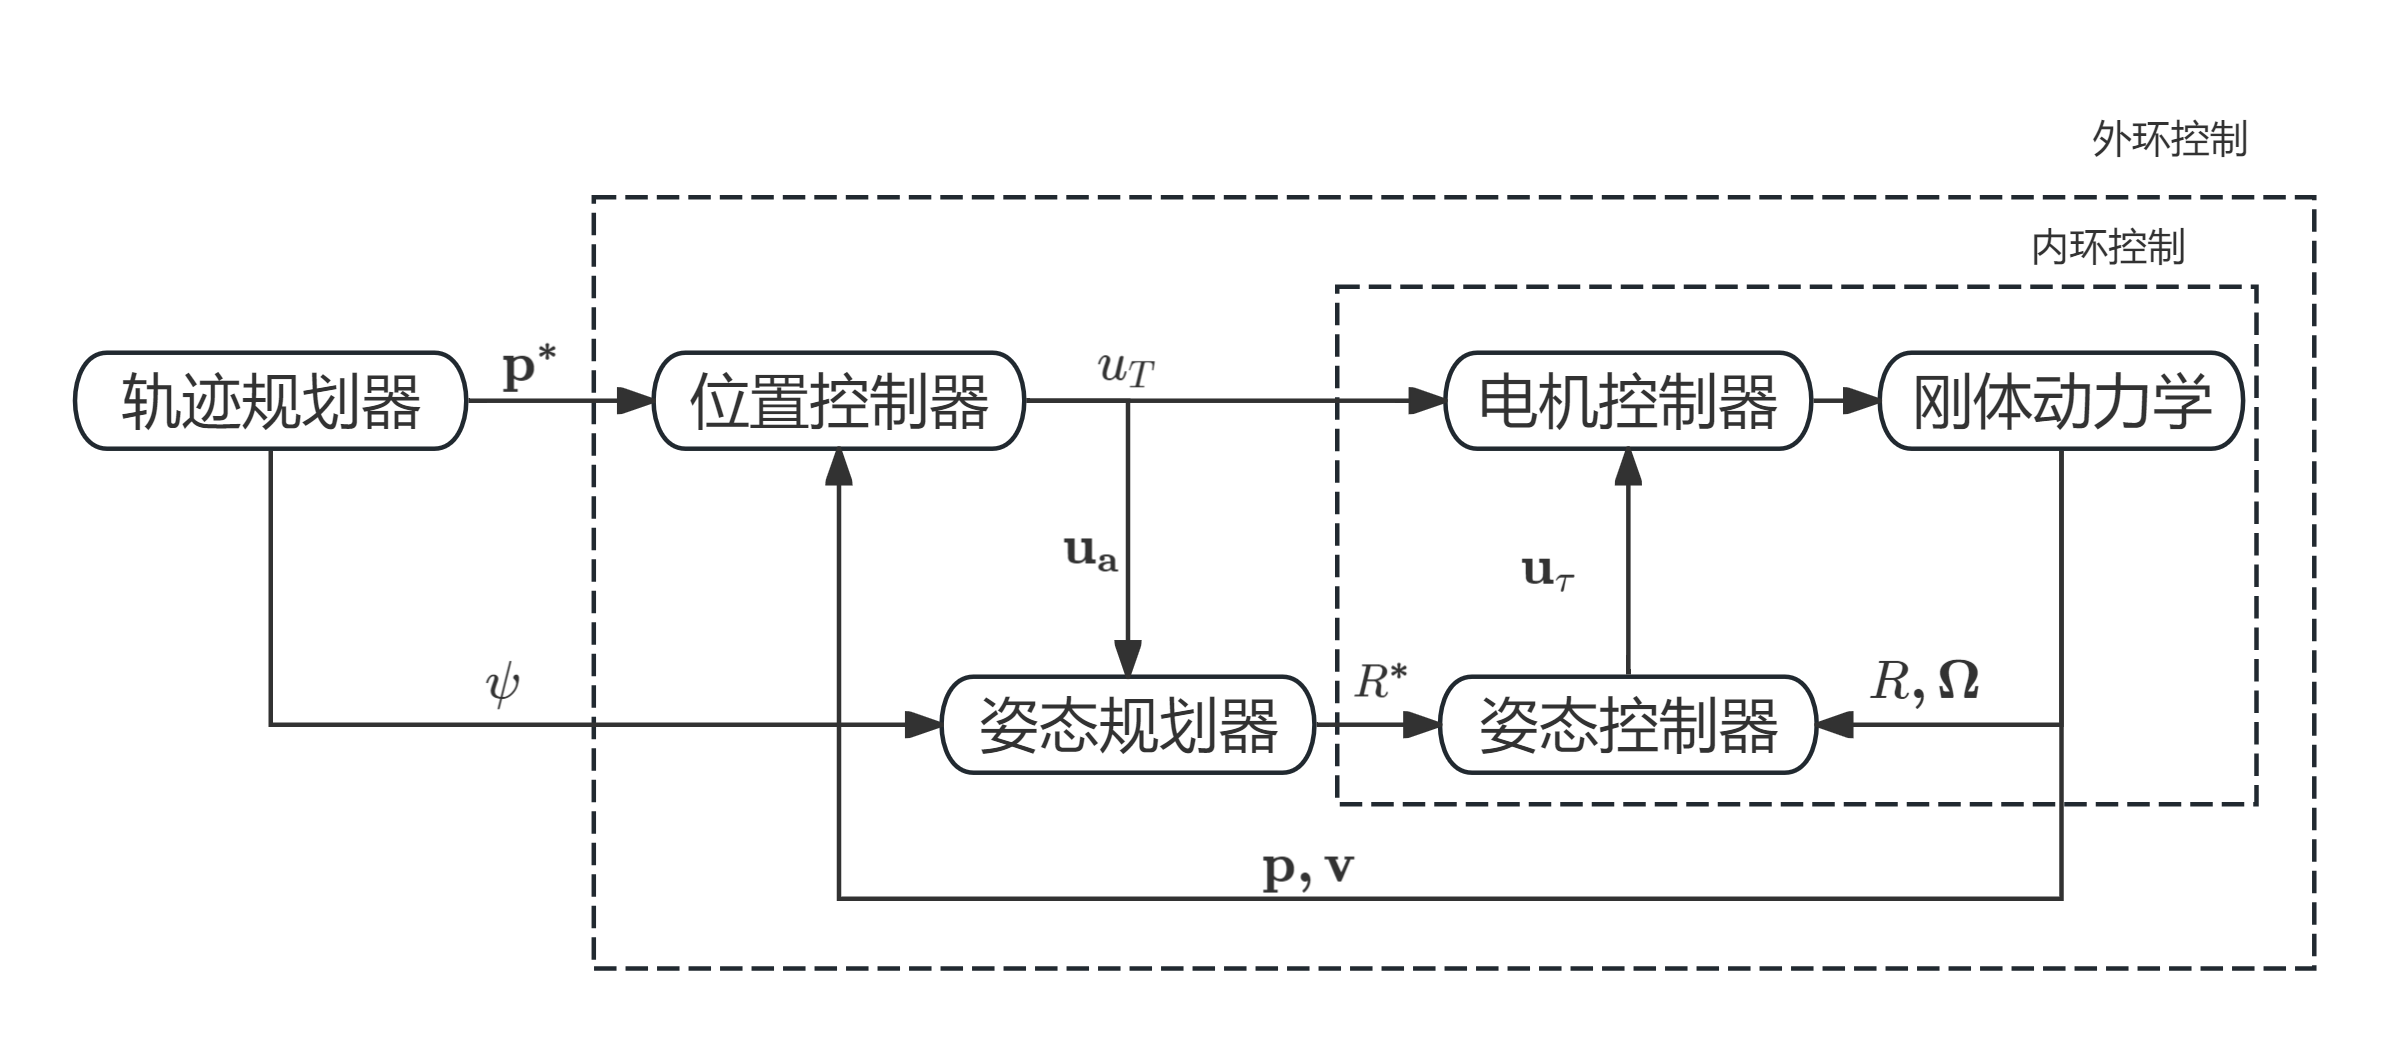
\includegraphics[width=0.8\linewidth]{images/2-2}
	\caption{四旋翼无人机分层控制结构}
	\label{四旋翼无人机分层控制结构}
	%\vspace{-20pt}
\end{figure}

在四旋翼无人机的分层控制架构中，电机控制环构成了最内层、最高带宽的执行单元。其核心任务是精确且快速地驱动各旋翼达到由上层姿态控制器所指定的期望转速。绝大多数四旋翼平台采用无刷直流电机，并通过高频脉宽调制信号进行电压控制。为克服电池电压衰减及气动负载变化带来的影响，通常采用单输入单输出的闭环控制策略，结合比例控制与前馈补偿项，以实现对期望转速的高精度跟踪。该控制环路的性能至关重要，其高带宽响应特性使得上层控制器可以将复杂的电机-旋翼动力学视为一个理想的执行器，从而为姿态与位置控制的解耦设计提供了基础。

在四旋翼无人机的分层控制架构中，姿态控制内环负责稳定并跟踪期望的姿态 $R^{*}(t)$。给定期望姿态 ${R}^*$，首先需要定义一个合适的姿态误差度量：
\begin{equation}
	{e_R}_\times = \frac{1}{2} ((R^*)^\top R - R^\top R^*), \label{姿态误差度量}
\end{equation}
该反对称矩阵物理意义明确，其对应的向量形式表征了当前姿态系${R}$相对于期望姿态系${R}^*$的旋转轴，且模长与旋转角的正弦值成正比。为推导线性控制器，以标称悬停位置为基准对动力学进行线性化处理，此时滚转角和俯仰角接近于零，角速度也接近于零。在 $ (0,0,\psi_0) $附近对旋转矩阵进行线性化。令$ {R}^* = {}_b^\omega R(\delta_\phi, \delta_\theta, \delta_\psi + \psi_0) $ 以及 $ R = {}_b^\omega R(0,0,\psi_0)$ ，公式(\ref{姿态误差度量})的近似形式如下：
\begin{equation}
	{e_R}_\times = 
	\begin{bmatrix}
		0 & \delta_\psi & -\delta_\theta \\
		-\delta_\psi & 0 & \delta_\phi \\
		\delta_\theta & -\delta_\phi & 0
	\end{bmatrix}
\end{equation}


基于此误差，可设计一个比例-微分控制律来生成所需的控制力矩 $\mathbf{u}_\tau$：
\begin{equation}
	\mathbf{u}_\tau = -k_R e_R - k_\Omega {e}_\Omega, \label{控制力矩}
\end{equation}
其中 ${e}_\Omega = \boldsymbol{\Omega} - \boldsymbol{\Omega}^*$ 是角速度误差，且通常期望角速度 $\boldsymbol{\Omega}^* $等于0。$k_R$ 和 $k_\Omega$ 为正定增益矩阵。该控制律通过负反馈作用，驱动姿态误差和角速度误差收敛至零，可确保系统在悬停位置附近发生微小偏差时仍保持稳定。为获得偏离悬停位置较大偏差时的收敛性，需回归至式(\ref{姿态误差度量})且不进行线性化处理。这使我们能够直接计算$ \mathrm{SO}(3) $上的误差。通过补偿非线性惯性项并纳入正确的误差项，可得到控制律：
\begin{equation}
	\mathbf{u}_\tau = 
	-k_e e_R - k_\Omega e_\Omega + 
	\boldsymbol{\Omega} \times J \boldsymbol{\Omega}
	- J ({\boldsymbol{\Omega}_\times}  R^\top R^* {\boldsymbol{\Omega}}^* - R^\top R^* \dot{\boldsymbol{\Omega}}^*) .
\end{equation}
该控制器几乎对任何旋转都保证具有指数稳定性\cite{5717652}。在悬停或低速巡航状态下，角速度 $\boldsymbol{\Omega}$ 及其导数项较小，科氏力与陀螺力矩项的影响处于次要地位。为降低工程实现的计算复杂度，上述控制律中的非线性补偿项（最后三项）通常可予以忽略，简化后的 PD 控制律即可满足大部分飞行任务的稳定性需求\cite{5980409}。

现在讨论关于四旋翼无人机质点轨迹$\mathbf{p}^{*}(t)$的跟踪控制问题。通过将动力学系统线性化来研究线性控制器，其中 $ \mathbf{p} = \mathbf{p}^{*}(t) , \dot{\mathbf{p}} = \mathbf{0}_3, \theta = \phi = 0, \psi = \psi^*(t) , \dot{\theta} = \dot{\phi} = \dot{\psi} = 0$ ，给定名义输入$ u_T = mg , \mathbf{u}_\tau = \mathbf{0}_3$ 对式(\ref{位置导数等于速度})进行线性化处理，可以得到：
\begin{align}
	\ddot{p_x} &= g(\delta\theta \mathbf{c}_{\psi^*} + \delta\phi \mathbf{s}_{\psi^*})\label{x方向加速度}, \\ 
	\ddot{p_y} &= g(\delta\theta \mathbf{s}_{\psi^*} - \delta\phi \mathbf{c}_{\psi^*})\label{y方向加速度}, \\ 
	\ddot{p_z} &= \frac{1}{m} u_T - g \label{z方向加速度}. 
\end{align}
为使轨迹位置误差的三个分量呈指数级收敛，需要使加速度向量$ \ddot{\mathbf{p}} $满足：
\begin{equation}
	(\ddot{\mathbf{p}}^{*}(t) - \ddot{\mathbf{p}}) + 
	k_d (\dot{\mathbf{p}}^{*}(t) - \dot{\mathbf{p}}) + 
	k_p ({\mathbf{p}^{*}(t)} - {\mathbf{p}}) = 0 .
\end{equation}
式中$ k_d, k_p$ 为增益矩阵。根据式(\ref{z方向加速度}), 可以得到推力指令$u_T$ ：
\begin{equation}
	u_T = m(g + {\ddot{p}_z}^*(t) + 
	k_{d,z} ( {\dot{p}_z}^*(t) - {\dot{p}_z}) + 
	k_{p,z} ({p_z}^*(t) - p_z)   ),
\end{equation}
用以保证位置误差 $ {{p}_z}-{{p}_z}^*(t) $随时间趋于零。同样对于其他两个期望加速度分量，可以根据公式(\ref{x方向加速度})和(\ref{y方向加速度}) 推导出期望的姿态角$ \phi^*,\theta^* $保证位置误差指数收敛：
\begin{align}
	\phi^* &= \frac{1}{g} (u_{a,x} \mathbf{s}_{\psi^*} - u_{a,y} \mathbf{c}_{\psi^*}) , \\
	\theta^* &= \frac{1}{g} (u_{a,x} \mathbf{c}_{\psi^*} + u_{a,y} \mathbf{s}_{\psi^*}) .
\end{align}
最终，$ (\phi^*, \theta^*, \psi) $被设定为姿态控制器的设定值。如图\ref{四旋翼无人机分层控制结构}所示，该控制问题通过解耦位置控制（外环）与姿态控制（内环）子问题来实现，其中位置控制回路为姿态控制器(\ref{控制力矩})提供姿态设定值，生成扭矩指令传递给最底层电机控制器执行。


\subsection{四旋翼无人机模型的线性化}

在无人机集群协同控制的研究中，通常采用分层控制架构。鉴于底层姿态控制回路的响应频率远高于顶层位置控制回路，根据时间尺度分离原则，可以合理假设底层姿态控制器能够实现对期望姿态指令的快速、无静差跟踪。因此，在设计顶层编队协同控制器时，可忽略四旋翼无人机复杂的姿态动力学耦合与非线性特性，将其视为三维空间中受控运动的质点，即对四旋翼无人机模型进行质点建模。

基于上述假设，第 $i$ 架无人机（$i = 1, \dots, N$）的平移动力学可简化为二阶积分器模型。定义 $\mathbf{p}_i(t) \in \mathbb{R}^m$ 和 $\mathbf{v}_i(t) \in \mathbb{R}^m$ 分别为第 $i$ 架无人机在惯性系下的位置向量和速度向量，其中 $m$ 为空间维度（通常 $m=2$ 或 $m=3$）。则系统的动力学方程可描述为：
\begin{equation}
	\begin{cases}
		\dot{\mathbf{p}}_i(t) = \mathbf{v}_i(t) \\
		\dot{\mathbf{v}}_i(t) = \mathbf{u}_i(t)
	\end{cases}
	\label{eq:double_integrator_dynamic}
\end{equation}
其中，$\mathbf{u}_i(t) \in \mathbb{R}^m$ 为第 $i$ 架无人机的控制输入向量，物理意义为虚拟加速度指令。该指令由顶层编队控制器生成，并通过逆动力学映射转化为底层飞控所需的推力与姿态角指令。

为了便于应用现代控制理论进行协同算法设计，将式(\ref{eq:double_integrator_dynamic})转化为连续时间的线性状态空间方程形式。定义第 $i$ 架无人机的状态向量 $\mathbf{x}_i \in \mathbb{R}^{2m}$ 为：
\begin{equation}
	\mathbf{x}_i = 
	\begin{bmatrix}
		\mathbf{p}_i \\
		\mathbf{v}_i
	\end{bmatrix}.
\end{equation}

结合式(\ref{eq:double_integrator_dynamic})，第 $i$ 个智能体的状态空间方程可表示为：
\begin{equation}
	\dot{\mathbf{x}}_i = A \mathbf{x}_i + B \mathbf{u}_i,
	\label{eq:state_space_single}
\end{equation}
其中，系统矩阵 $A \in \mathbb{R}^{2m \times 2m}$ 与输入矩阵 $B \in \mathbb{R}^{2m \times m}$ 分别定义为：
\begin{equation}
	A = 
	\begin{bmatrix}
		\mathbf{0}_m & \mathbf{I}_m \\
		\mathbf{0}_m & \mathbf{0}_m
	\end{bmatrix}, \quad
	B = 
	\begin{bmatrix}
		\mathbf{0}_m \\
		\mathbf{I}_m
	\end{bmatrix}.
\end{equation}
上式中，$\mathbf{I}_m$ 表示 $m$ 维单位矩阵，$\mathbf{0}_m$ 表示 $m$ 维全零矩阵。

对于包含 $N$ 架无人机的整个集群系统，通过定义全局状态向量 $\mathbf{x} = [\mathbf{x}_1^\top, \dots, \mathbf{x}_N^\top]^\top \in \mathbb{R}^{2mN}$ 和全局输入向量 $\mathbf{u} = [\mathbf{u}_1^\top, \dots, \mathbf{u}_N^\top]^\top \in \mathbb{R}^{mN}$，集群整体的动力学模型可写为 Kronecker 积形式：
\begin{equation}
	\dot{\mathbf{x}} = (I_N \otimes A) \mathbf{x} + (I_N \otimes B) \mathbf{u}.
	\label{eq:state_space_global}
\end{equation}
式(\ref{eq:state_space_single})与式(\ref{eq:state_space_global})所描述的线性连续二阶积分器系统，保留了位置与速度之间的核心运动学约束，结构简洁且具有完全能控性，为后续章节中分布式观测器与编队控制协议的设计提供了标准的模型基础。




\section{代数图论与刚性图理论基础}
\label{sec:graph_and_rigidity}

无人机集群的分布式协同控制高度依赖于个体间的信息交互网络。在数学描述上，代数图论为刻画集群通信拓扑提供了标准语言，而刚性图理论则为解决基于距离或方位的编队队形保持与定位问题提供了严谨的几何约束判据。本节将分别从通信拓扑描述与几何构型约束两个维度展开讨论。

\subsection{代数图论基础}
令 $\mathcal{G} = (\mathcal{V}, \mathcal{E})$ 表示一个包含 $N$ 个节点的图，用于描述无人机集群的通信拓扑。其中，节点集合 $\mathcal{V} = \{1, 2, \dots, N\}$ 代表集群中的 $N$ 架无人机，边集合 $\mathcal{E} \subseteq \mathcal{V} \times \mathcal{V}$ 代表无人机之间的通信链路或传感关系，边的总数量记为 $M = |\mathcal{E}|$。若无人机 $j$ 能够向无人机 $i$ 发送信息，则存在一条边 $(i, j) \in \mathcal{E}$。此时，称节点 $j$ 为节点 $i$ 的邻居，节点 $i$ 的邻居集合记为 $\mathcal{N}_i = \{j \in \mathcal{V} \mid (i, j) \in \mathcal{E},i \neq j\}$。图的代数性质主要通过以下几类矩阵来刻画：

\textbf{（1）邻接矩阵：} $\mathcal{A} \in \mathbb{R}^{N \times N}$ 是描述图中节点间连接强度的基础矩阵。对于无权图，若 $(i, j) \in \mathcal{E}$，则 $a_{ij} = 1$，否则 $a_{ij} = 0$。对于加权图，其元素定义为：
\begin{equation}
	a_{ij} = 
	\begin{cases}
		w_{ij}, & \text{若 } (i, j) \in \mathcal{E} \\
		0, & \text{其他}
	\end{cases},
\end{equation}
其中 $w_{ij} > 0$ 为边的权重，通常用于表示通信质量或传感置信度。我们规定图中无自环，即 $a_{ii} = 0$。

\textbf{（2）度矩阵：} $\mathcal{D} = \text{diag}\{d_1, \dots, d_N\}$ 是一个对角矩阵，反映了节点的局部连接规模。其中 $d_i$ 为节点 $i$ 的入度，定义为 $d_i = \sum_{j=1}^{N} a_{ij}$。对于无向图，入度等于出度。

\textbf{（3）关联矩阵：} $\mathcal{H} \in \mathbb{R}^{N \times M}$ 描述了节点与边的拓扑关系。对于任意给定的边方向定向，若第 $k$ 条边 $e_k = (i, j)$ 连接节点 $j$ 指向节点 $i$（$j \to i$），则关联矩阵的第 $k$ 列元素定义为：
\begin{equation}
	h_{ik} = 
	\begin{cases}
		1, & \text{若节点 } i \text{ 为边 } e_k \text{ 的头节点} \\
		-1, & \text{若节点 } i \text{ 为边 } e_k \text{ 的尾节点} \\
		0, & \text{其他}
	\end{cases}.
\end{equation}
关联矩阵的每一列恰好包含一个 $1$ 和一个 $-1$，其余元素为 $0$。

\textbf{（4）拉普拉斯矩阵：} $\mathcal{L} \in \mathbb{R}^{N \times N}$ 是图论在控制领域应用最广泛的矩阵，定义为度矩阵与邻接矩阵之差：
\begin{equation}
	\mathcal{L} = \mathcal{D} - \mathcal{A}.
\end{equation}
对于边权为1的无向图，拉普拉斯矩阵可由关联矩阵表示为 $\mathcal{L} = \mathcal{H} \mathcal{H}^\top$。这一性质揭示了拉普拉斯矩阵半正定性的代数本质。对于无向图，若图 $\mathcal{G}$ 包含一棵生成树，则 $\mathcal{L}$ 具有唯一的零特征值，其余特征值均大于零。其最小非零特征值 $\lambda_2(\mathcal{L})$ 被称为代数连通度，数值越大，网络连通性越强，编队系统的一致性收敛速度越快。

\subsection{刚性图理论}
本小节针对刚性图理论展开讨论，主要参考\parencite{Hendrickson1992Conditions,Anderson2010FormalTO}文献。在非全维位置量测的条件下，编队队形能否保持唯一确定，取决于底层的几何约束结构。刚性图理论主要研究由节点和边构成的框架在保持边长不变的情况下，其几何形状是否具有抗形变能力。一个框架定义为 $(\mathcal{G}, \mathbf{p})$，其中 $\mathcal{G}$ 为图拓扑，$\mathbf{p} = [\mathbf{p}_1^\top, \dots, \mathbf{p}_N^\top]^\top \in \mathbb{R}^{Nn}$ 为所有节点在 $n$ 维空间中的堆叠坐标向量。

刚性矩阵是判定无穷小刚性的核心工具。对于任意一条边 $(i, j) \in \mathcal{E}$，其长度约束满足欧氏距离方程 $||\mathbf{p}_i - \mathbf{p}_j||^2 = c_{ij}$。对该约束关于时间求导，可得一阶微分约束：
\begin{equation}
	(\mathbf{p}_i - \mathbf{p}_j)^\top (\dot{\mathbf{p}}_i - \dot{\mathbf{p}}_j) = 0.
\end{equation}
将所有 $M$ 条边的微分约束写成紧凑的矩阵形式，即 $\mathcal{R}(\mathbf{p}) \dot{\mathbf{p}} = \mathbf{0}$，其中 $\mathcal{R}(\mathbf{p}) \in \mathbb{R}^{M \times Nn}$ 即为刚性矩阵。$\mathcal{R}(\mathbf{p})$ 的每一行对应一条边，每一列对应一个节点的坐标分量。对于连接节点 $i$ 和 $j$ 的行，其在节点 $i$ 和 $j$ 对应的列上的非零块分别为 $(\mathbf{p}_i - \mathbf{p}_j)^\top$ 和 $(\mathbf{p}_j - \mathbf{p}_i)^\top$，其余位置为零。

一阶刚性又称无穷小刚性。若框架 $(\mathcal{G}, \mathbf{p})$ 的所有满足 $\mathcal{R}(\mathbf{p}) \dot{\mathbf{p}} = \mathbf{0}$ 的无穷小运动 $\dot{\mathbf{p}}$ 仅包含刚体整体平移和旋转运动，而不包含任何非刚性形变，则称该框架具有一阶刚性。在 $n$ 维欧氏空间中，刚体运动的自由度为 $\frac{n(n+1)}{2}$（包含 $n$ 个平移自由度和 $\frac{n(n-1)}{2}$ 个旋转自由度）。因此，判定一阶刚性的充要条件是刚性矩阵 $\mathcal{R}(\mathbf{p})$ 的秩达到系统最大可能的约束秩。具体而言，其秩条件满足：
\begin{equation}
	\text{rank}(\mathcal{R}(\mathbf{p})) = 
	\begin{cases}
		Nn - \frac{n(n+1)}{2}, & \text{若 } N \ge n \\
		\frac{N(N-1)}{2}, & \text{若 } N < n
	\end{cases}.
\end{equation}
上式中的第一种情况对应于通常的编队规模，即节点数量足以张成 $n$ 维空间。第二种情况$ N < n$则对应于退化情形，此时节点无法张成满维空间，例如三维空间中的 2 个点只能形成一条线段，要实现刚性必须形成完全图，即所有节点间均有边相连，此时秩等于边数。

最小刚性是指一个刚性框架在移除任意一条边后即变为非刚性的临界状态。在代数层面上，这意味着刚性矩阵 $\mathcal{R}(\mathbf{p})$ 不仅满足上述刚性秩条件，且其所有行向量线性无关。
特别地，在二维情形下，Laman 条件给出了图具有最小刚性的组合充要条件：图 $\mathcal{G}$ 的边数恰为 $2N-3$，且对于任意包含 $N' \ge 2$ 个节点的子图，其边数不超过 $2N' - 3$。最小刚性结构在工程应用中具有重要意义。它能够在保证编队几何构型唯一性的前提下，将所需的通信链路或传感器数量降至最低，从而有效降低系统的通信负载与计算复杂度。有关刚性矩阵的更多解释可以参考文献\parencite{4653105}。

\section{本章小结}

本章主要针对无人机集群协同控制任务，建立了系统动力学模型与网络拓扑模型，为后续的控制器设计与理论分析奠定了基础。主要工作总结如下：

首先，针对四旋翼无人机动力学系统的欠驱动、强耦合与非线性特性，采用了分层控制的建模思想。通过分析时间尺度分离特性，假设底层姿态环具有理想的快速跟踪性能，将复杂的六自由度刚体动力学模型简化为位置环的二阶积分器模型。该线性化模型在保留无人机位置运动核心特征的同时，显著降低了协同控制律设计的复杂度。

其次，引入代数图论作为描述集群通信拓扑的数学语言。定义了邻接矩阵、拉普拉斯矩阵及关联矩阵，建立了节点间信息交互的代数描述框架。针对本文关注的非全维位置量测问题，引入了刚性图理论，详细阐述了刚性矩阵的构造方法、一阶刚性的秩判据以及最小刚性结构的性质。刚性图理论揭示了在仅有距离或相对方位约束下编队队形保持的几何本质，为分析非全维量测下的系统可观测性以及设计分布式状态观测器提供了关键的理论支撑。

综上所述，本章构建的“二阶积分器动力学-刚性图拓扑”一体化建模框架，有效解决了从物理实体到数学抽象的映射问题，明确了协同控制问题的数学描述形式。